\documentclass[tikz, border=10pt]{standalone}
\usepackage{amsmath}
\usetikzlibrary{calc}
\begin{document}
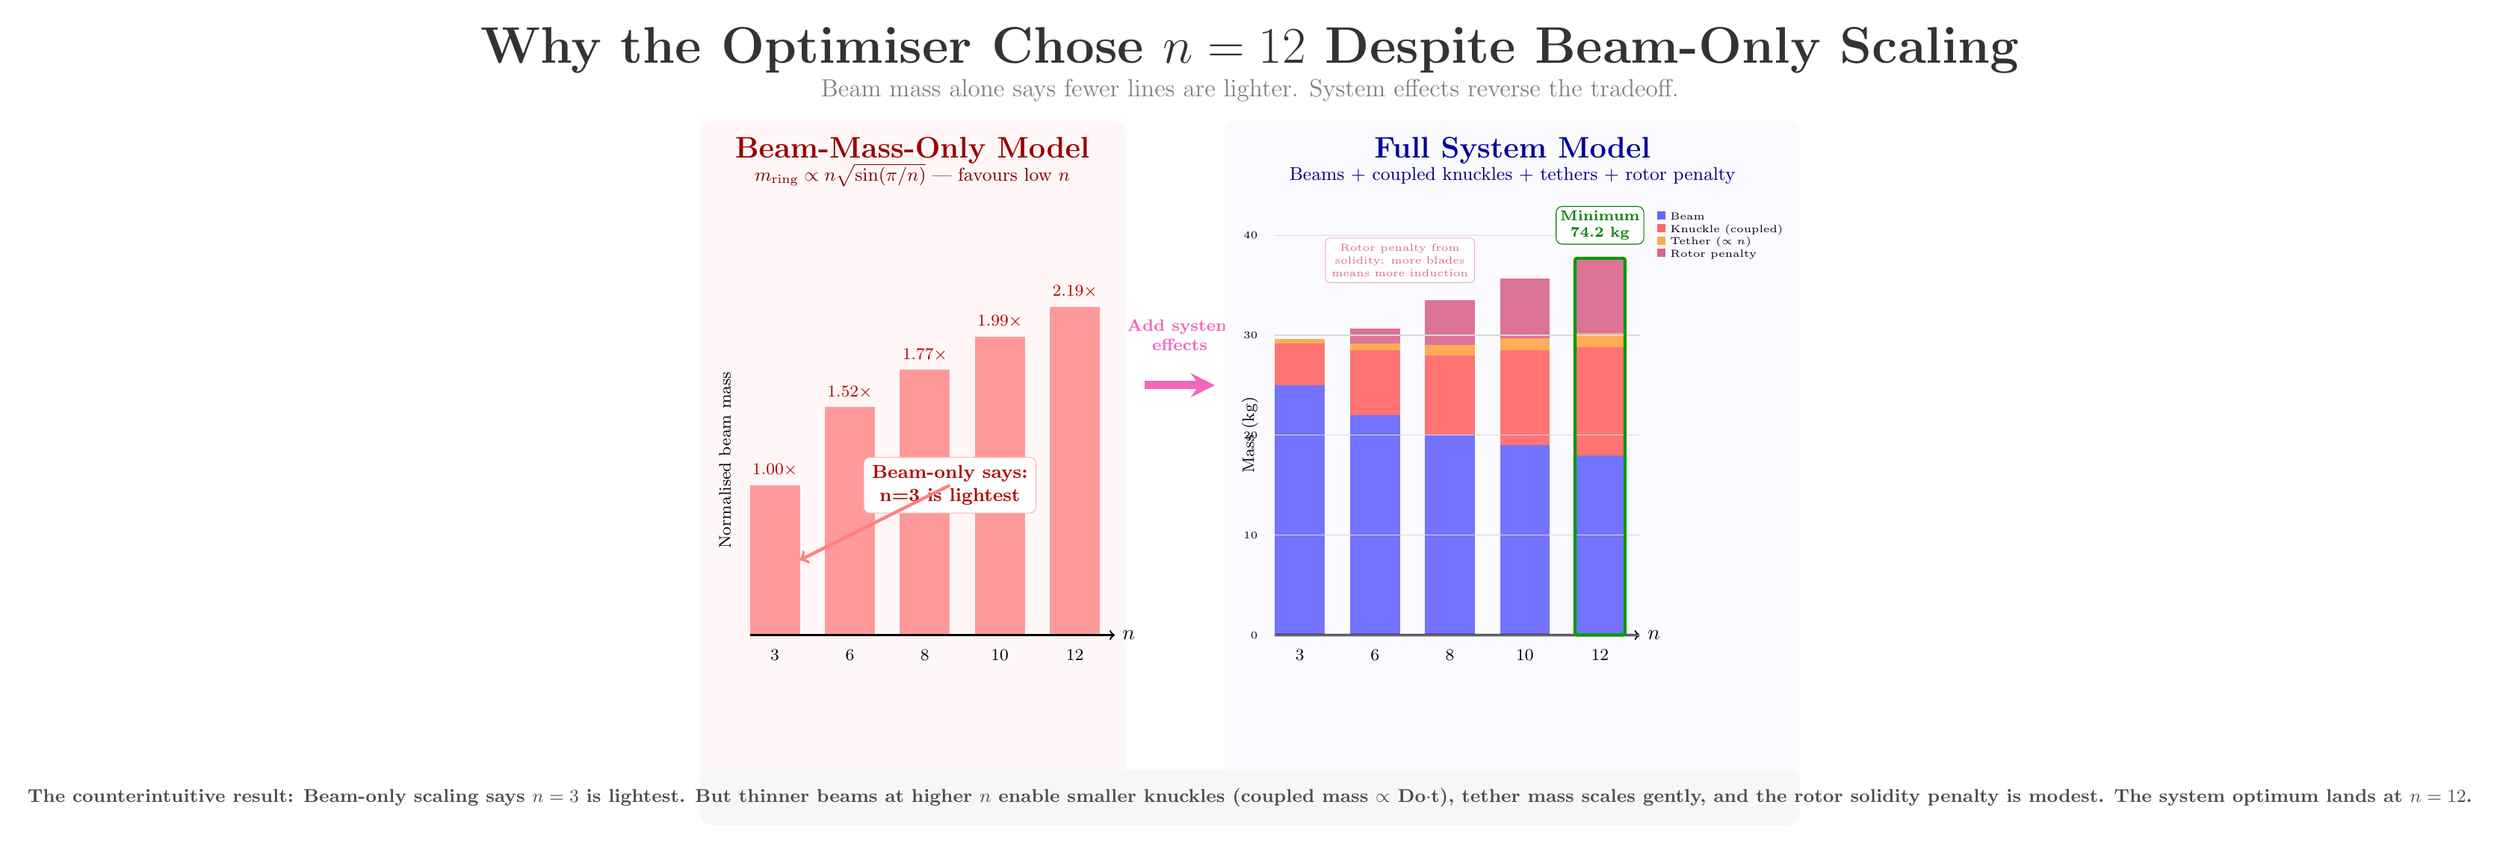
\begin{tikzpicture}[scale=0.85]

% === GLOBAL TITLE ===
\node[font=\bfseries\Huge, black!80] at (10.5,13.2) {Why the Optimiser Chose $n=12$ Despite Beam-Only Scaling};
\node[font=\large, black!50] at (10.5,12.4) {Beam mass alone says fewer lines are lighter. System effects reverse the tradeoff.};

% === LEFT: Beam-only model ===
\begin{scope}[shift={(0,0)}]
  \fill[red!3, rounded corners=6pt] (-0.5,-2.0) rectangle (8.0,11.8);
  \node[font=\bfseries\Large, red!60!black] at (3.75,11.2) {Beam-Mass-Only Model};
  \node[font=\small, red!50!black] at (3.75,10.7) {$m_{\text{ring}} \propto n\sqrt{\sin(\pi/n)}$ --- favours low $n$};

  % Bars: normalized beam mass
  % n=3:1.00, n=6:1.52, n=8:1.77, n=10:1.99, n=12:2.19
  \foreach \n/\val/\label/\i in {3/1.00/1.00/0, 6/1.52/1.52/1, 8/1.77/1.77/2, 10/1.99/1.99/3, 12/2.19/2.19/4} {
    \pgfmathsetmacro{\barht}{\val * 3.0}
    \pgfmathsetmacro{\x}{1.0 + \i * 1.5}
    \fill[red!40] ({\x-0.5}, 1.5) rectangle ({\x+0.5}, {1.5+\barht});
    \node[font=\footnotesize, red!70!black] at (\x, {1.5+\barht+0.3}) {\label$\times$};
  }

  \draw[->, thick] (0.5,1.5) -- (7.8,1.5) node[right, font=\bfseries] {$n$};
  \foreach \n/\i in {3/0, 6/1, 8/2, 10/3, 12/4} { \node[font=\footnotesize] at ({1.0+\i*1.5}, 1.1) {\n}; }
  \node[font=\footnotesize, rotate=90] at (0.0,5.0) {Normalised beam mass};

  % Annotation
  \node[font=\small\bfseries, red!70!black, align=center, fill=white, draw=red!30, rounded corners=3pt, inner sep=4pt] at (4.5,4.5) {Beam-only says:\\\textbf{n=3 is lightest}};
  \draw[->, red!50, line width=1.5pt] (4.5,4.5) -- (1.5,3.0);
\end{scope}

% === BRIDGE ===
\draw[->, line width=4pt, >=stealth, magenta!60] (8.4,6.5) -- (9.8,6.5);
\node[font=\bfseries\footnotesize, magenta!60, align=center] at (9.1,7.5) {Add system\\effects};

% === RIGHT: System model ===
\begin{scope}[shift={(10.5,0)}]
  \fill[blue!2, rounded corners=6pt] (-0.5,-2.0) rectangle (11.0,11.8);
  \node[font=\bfseries\Large, blue!60!black] at (5.25,11.2) {Full System Model};
  \node[font=\small, blue!50!black] at (5.25,10.7) {Beams + coupled knuckles + tethers + rotor penalty};

  % System mass components (kg scale)
  % n: beam, knuckle, tether, rotor
  \foreach \n/\beam/\knuckle/\tether/\rotor/\i in {
    3/25/4.2/0.4/0/0,
    6/22/6.5/0.7/1.5/1,
    8/20/8.0/1.0/4.5/2,
    10/19/9.5/1.2/6.0/3,
    12/18/10.8/1.4/7.5/4
  } {
    \pgfmathsetmacro{\x}{1.0 + \i * 1.5}
    \fill[blue!55] ({\x-0.5}, 1.5) rectangle ({\x+0.5}, {1.5+\beam*0.2});
    \fill[red!55] ({\x-0.5}, {1.5+\beam*0.2}) rectangle ({\x+0.5}, {1.5+\beam*0.2+\knuckle*0.2});
    \fill[orange!65] ({\x-0.5}, {1.5+\beam*0.2+\knuckle*0.2}) rectangle ({\x+0.5}, {1.5+\beam*0.2+\knuckle*0.2+\tether*0.2});
    \fill[purple!55] ({\x-0.5}, {1.5+\beam*0.2+\knuckle*0.2+\tether*0.2}) rectangle ({\x+0.5}, {1.5+\beam*0.2+\knuckle*0.2+\tether*0.2+\rotor*0.2});
  }

  \draw[->, thick] (0.5,1.5) -- (7.8,1.5) node[right, font=\bfseries] {$n$};
  \foreach \n/\i in {3/0, 6/1, 8/2, 10/3, 12/4} { \node[font=\footnotesize] at ({1.0+\i*1.5}, 1.1) {\n}; }

  % Y-axis ticks (kg)
  \foreach \y/\label in {1.5/0, 3.5/10, 5.5/20, 7.5/30, 9.5/40} {
    \draw[gray!30] (0.5,\y) -- (7.8,\y);
    \node[left, font=\tiny] at (0.3,\y) {\label};
  }
  \node[font=\footnotesize, rotate=90] at (0.0,5.5) {Mass (kg)};

  % Legend
  \node[font=\tiny, align=left, anchor=west] at (8.0,9.5) {
    \textcolor{blue!60}{\rule{4pt}{4pt}} Beam\\
    \textcolor{red!60}{\rule{4pt}{4pt}} Knuckle (coupled)\\
    \textcolor{orange!70}{\rule{4pt}{4pt}} Tether ($\propto n$)\\
    \textcolor{purple!60}{\rule{4pt}{4pt}} Rotor penalty};

  % Optimum marker
  \draw[green!60!black, line width=1.5pt, rounded corners=1pt] (6.5, 1.5) rectangle (7.5, 9.04);
  \node[font=\bfseries\scriptsize, green!50!black, fill=white, draw=green!50!black, rounded corners=3pt, inner sep=2pt, align=center] at (7.0,9.7) {Minimum\\74.2 kg};

  % Rotor penalty annotation
  \node[font=\tiny, purple!60, align=center, fill=white, draw=purple!30, rounded corners=2pt, inner sep=3pt] at (3.0,9.0) {Rotor penalty from\\solidity: more blades\\means more induction};
\end{scope}

% === BOTTOM === 
\fill[black!3, rounded corners=6pt] (-0.5,-2.3) rectangle (21.5,-1.2);
\node[font=\small\bfseries, black!70, align=center] at (10.5,-1.75) {
  \textbf{The counterintuitive result:} Beam-only scaling says $n=3$ is lightest. But thinner beams at higher $n$ enable smaller knuckles
  (coupled mass $\propto$ Do$\cdot$t), tether mass scales gently, and the rotor solidity penalty is modest. The system optimum lands at $n=12$.};

\end{tikzpicture}
\end{document}
